\section{Context}
Our system will target a work environment or an educational environment.
%The targeted environment is all work or educational environment.
The analysis and design process will be based upon a university, but the system should be easily implemented at any other work environment. 

\begin{figure}[H]%
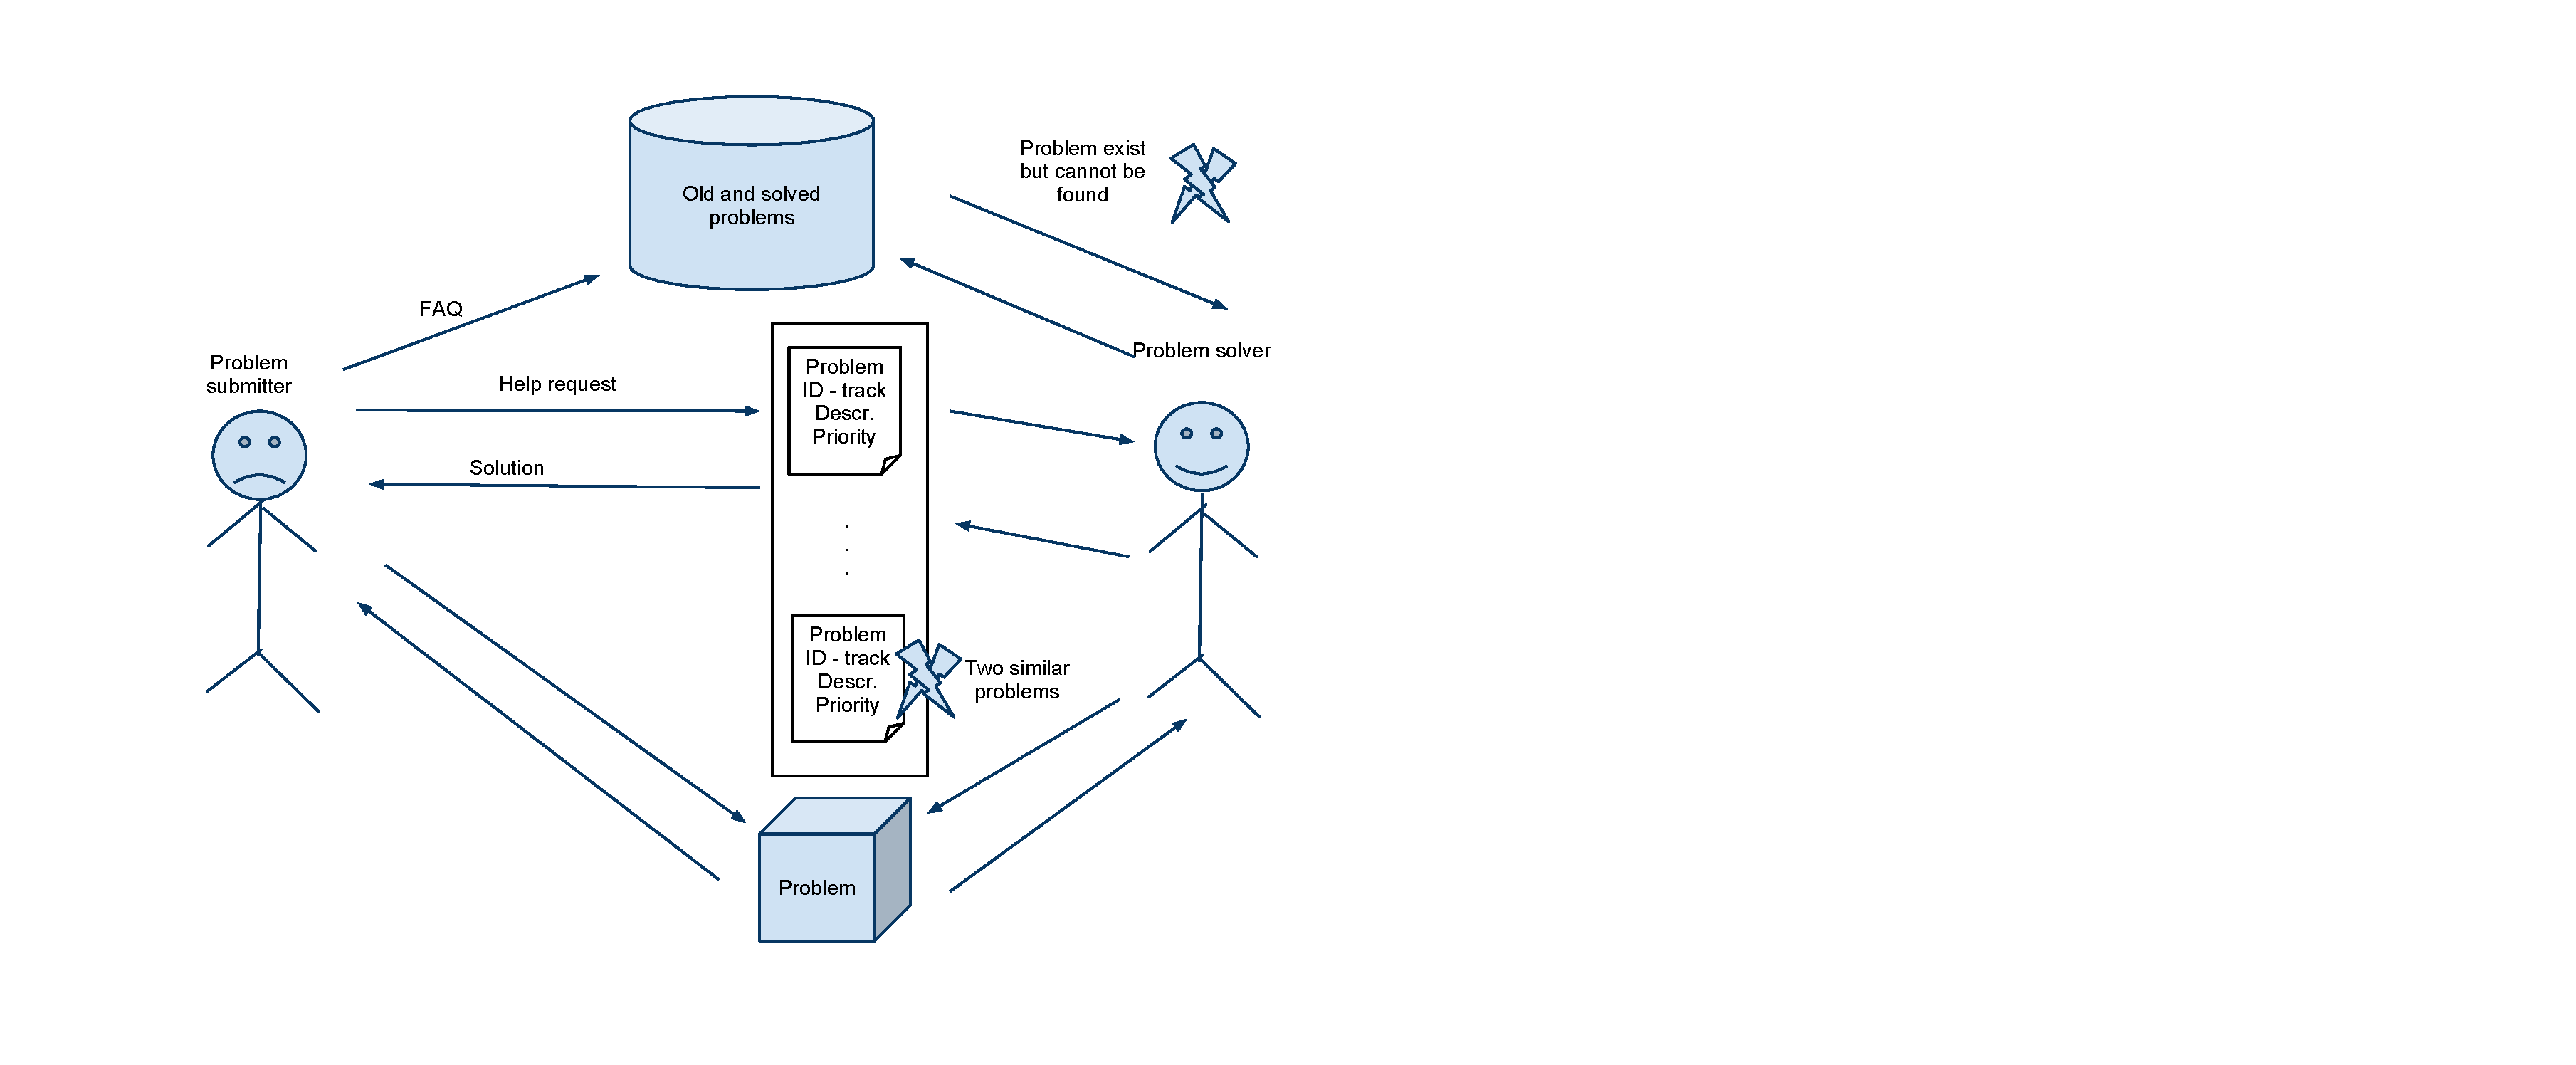
\includegraphics[scale = 0.45]{input/background/rich_picture.pdf}%
\morscaption{Rich picture of our system}%
\label{fig:rich_picture}%
\end{figure}

To fully understand the context we draw a rich picture which can be seen on figure \ref{fig:rich_picture}. 
The central aspects on the rich picture is that both the problem submitter and the problem solver can act on the problem, but will communicate through the system. 
From the rich picture we see a few conflicts in the environment. 
The first is that problem exist but cannot be found.
The second is that there could exist two similar problem.
The central objects in the system are the problems and solutions.

\subsection{Problem Domain}
A central phenomena in our system will be to add a problem to the system.
This will occur when a client finds a problem in the organization and wants to submit it, in order to get it solved.
This phenomena will also include a staff member, namely the one who will initially be assigned to the problem.

Another important phenomena in our system is when a problem is solved.
This is initiated by a staff member and will result in a notification to the clients who are subscribing to the problem.
A client who submit the problem can suggest it to be reopened if he/she is not satisfied with the solution.

Chapter \ref{chap:problemDomain} gives a detailed analysis of the problem domain and will elaborate on the phenomena.

\subsection{Application Domain}
The people who will be acting on the system is the problem solver and submitter. Most likely the submitter will be a student in a university environment and the solver will be the technical staff. But the submitter could be a staff as well. Beside the two main actors there is an admin who can administrate the staff, clients, and the system itself.

A detailed analysis of the application domain is presented in chapter \ref{chap:app_domain}, where the actors and there use cases are further described.